%diagramma del package%
\subsection{premi/server}
\begin{figure}[H]
\begin{center}
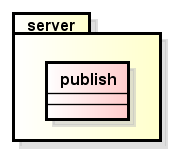
\includegraphics[scale=0.70]{img/diapkg/server.png}
\caption{Diagramma del package premi/client}
\end{center}
\end{figure}


%-------  diagramma della classe%
\subsubsection{premi/server/publish}
\begin{figure}[H]
\begin{center}
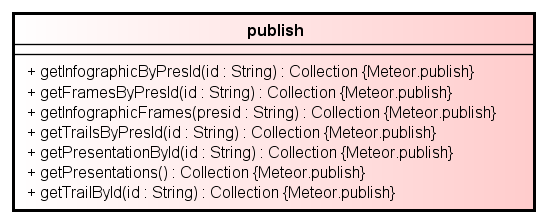
\includegraphics[scale=0.55]{img/diacla/publish.png}
\caption{Diagramma della classe premi/server/publish}
\end{center}
\end{figure}




\begin{description}
%-------  descrizione della classe%
\item[Descrizione] \hfill
	Lista di metodi che pubblicano al client solamente le informazioni a cui esso puo' accedere. Utilizzano tutti  \textbf{[Meteor.publish]} per rendere reperibili i metodi attraverso Meteor

	
	
%-------  lista dei metodi%	
\item[Metodi] \hfill
	
	% -- inizio metodo -- %
	\begin{description}
		\item[\textbf{\color{blue}+ getInfographicByPresId(id : String) : Collection			}] \hfill
			Pubblica una lista di infografiche associate ad una presentazione
			
		\begin{description}
			% -- lista argomenti del metodo -- %
			\item[Argomenti] \hfill
				\begin{itemize}
				
					\item \textbf{id : String			} \hfill
					Il codice identificativo della presentazione associata alle infografiche
					
				\end{itemize}
			% -- note aggiuntive sul metodo -- %
			\item[Note] \hfill
			\begin{itemize}
					\item Dev'essere inserito come funzione \textbf{publishfunction} in Meteor.publish
				\end{itemize}
		\end{description}
	\end{description}
	% -- fine metodo -- %
	
	% -- inizio metodo -- %
	\begin{description}
		\item[\textbf{\color{blue}+ getFramesByPresId(id : String) : Collection			}] \hfill
			Pubblica una lista di frames associati ad una presentazione
			
		\begin{description}
			% -- lista argomenti del metodo -- %
			\item[Argomenti] \hfill
				\begin{itemize}
				
					\item \textbf{id : String			} \hfill
					Il codice identificativo della presentazione associata ai frame
					
				\end{itemize}
			% -- note aggiuntive sul metodo -- %
			\item[Note] \hfill
			\begin{itemize}
					\item Dev'essere inserito come funzione \textbf{publishfunction} in Meteor.publish
					\item La presentazione deve appartenere all'utente che ha effettuato la richiesta
				\end{itemize}
		\end{description}
	\end{description}
	% -- fine metodo -- %
	
	% -- inizio metodo -- %
	\begin{description}
		\item[\textbf{\color{blue}+ getInfographicFrames(presid : String) : Collection			}] \hfill
			Pubblica una lista di tutti i frames delle infografiche di una presentazione
			
		\begin{description}
			% -- lista argomenti del metodo -- %
			\item[Argomenti] \hfill
				\begin{itemize}
				
					\item \textbf{presid : String			} \hfill
					Il codice identificativo della presentazione associata alle infografiche
					
				\end{itemize}
			% -- note aggiuntive sul metodo -- %
			\item[Note] \hfill
			\begin{itemize}
					\item Dev'essere inserito come funzione \textbf{publishfunction} in Meteor.publish
					\item La presentazione deve appartenere all'utente che ne ha effettuato la richiesta
				\end{itemize}
		\end{description}
	\end{description}
	% -- fine metodo -- %
	
	% -- inizio metodo -- %
	\begin{description}
		\item[\textbf{\color{blue}+ getTrailsByPresId(id : String) : Collection			}] \hfill
			Pubblica una lista di trails associati ad una presentazione
			
		\begin{description}
			% -- lista argomenti del metodo -- %
			\item[Argomenti] \hfill
				\begin{itemize}
				
					\item \textbf{id : String			} \hfill
					Il codice identificativo della presentazione associata ai trails
					
				\end{itemize}
			% -- note aggiuntive sul metodo -- %
			\item[Note] \hfill
			\begin{itemize}
					\item Dev'essere inserito come funzione \textbf{publishfunction} in Meteor.publish
					\item La presentazione deve appartenere all'utente che ne ha effettuato la richiesta
				\end{itemize}
		\end{description}
	\end{description}
	% -- fine metodo -- %
	
	% -- inizio metodo -- %
	\begin{description}
		\item[\textbf{\color{blue}+ getPresentationsById(id : String) : Collection			}] \hfill
			Pubblica una presentazione all'utente
			
		\begin{description}
			% -- lista argomenti del metodo -- %
			\item[Argomenti] \hfill
				\begin{itemize}
				
					\item \textbf{id : String			} \hfill
					Il codice identificativo della presentazione
					
				\end{itemize}
			% -- note aggiuntive sul metodo -- %
			\item[Note] \hfill
			\begin{itemize}
					\item Dev'essere inserito come funzione \textbf{publishfunction} in Meteor.publish
					\item La presentazione deve appartenere all'utente che ne ha effettuato la richiesta
				\end{itemize}
		\end{description}
	\end{description}
	% -- fine metodo -- %
	
	% -- inizio metodo -- %
	\begin{description}
		\item[\textbf{\color{blue}+ getPresentations() : Collection			}] \hfill
			Pubblica una lista di tutte le presentazioni che l'utente possiede
			
		\begin{description}
			
			% -- note aggiuntive sul metodo -- %
			\item[Note] \hfill
			\begin{itemize}
					\item Dev'essere inserito come funzione \textbf{publishfunction} in Meteor.publish
					\item Le presentazioni devono appartenere all'utente che ne ha effettuato la richiesta
				\end{itemize}
		\end{description}
	\end{description}
	% -- fine metodo -- %
	
	% -- inizio metodo -- %
	\begin{description}
		\item[\textbf{\color{blue}+ getTrailsById(id : String) : Collection			}] \hfill
			Pubblica un trail all'utente che ne ha effettuato la richiesta
			
		\begin{description}
			% -- lista argomenti del metodo -- %
			\item[Argomenti] \hfill
				\begin{itemize}
				
					\item \textbf{id : String			} \hfill
					Il codice identificativo del trail da pubblicare
					
				\end{itemize}
			% -- note aggiuntive sul metodo -- %
			\item[Note] \hfill
			\begin{itemize}
					\item Dev'essere inserito come funzione \textbf{publishfunction} in Meteor.publish
					\item Il trail deve appartenere all'utente che ne ha effettuato la richiesta
				\end{itemize}
		\end{description}
	\end{description}
	% -- fine metodo -- %
	
	
	
	
\end{description}










%-------  diagramma della classe%
\subsubsection{premi/server/methods}
\begin{figure}[H]
\begin{center}
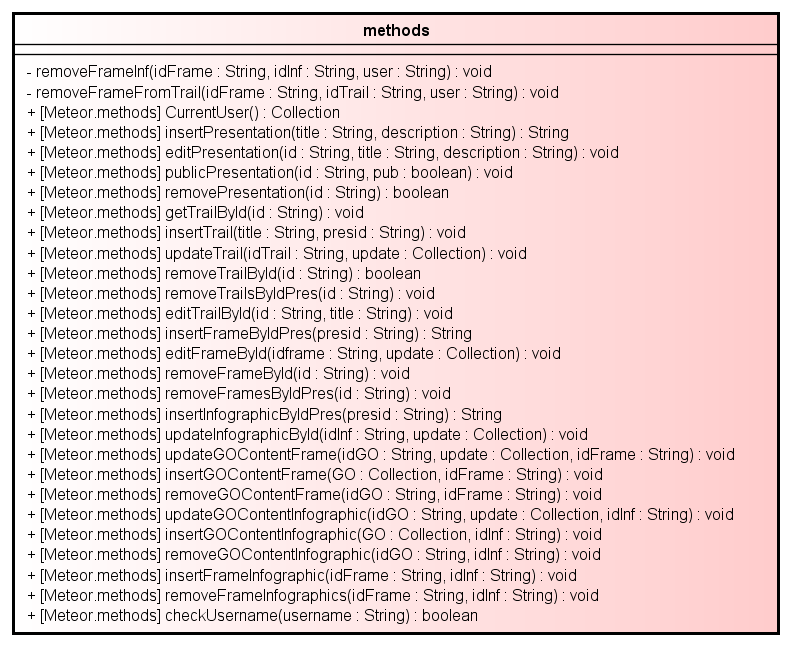
\includegraphics[scale=0.55]{img/diacla/methods.png}
\caption{Diagramma della classe premi/server/methods}
\end{center}
\end{figure}




\begin{description}
%-------  descrizione della classe%
\item[Descrizione] \hfill
	Lista di metodi che permettono al client di interagire con il database del server. I metodi marcati \textbf{[Meteor.methods]} devono essere inseriti nel servizio \$meteor per permettere poi al client di accedervi attraverso il pattern Dependency Injection$_G$






%-------  lista dei metodi%	
\item[Metodi] \hfill

	% -- inizio metodo -- %
	\begin{description}
		\item[\textbf{\color{blue}- removeFrameInf(idFrame : String, idInf : String, user : String) : void			}] \hfill
			Metodo privato di utilità che rimuove ogni occorrenza di un frame da un'infografica.
			
		\begin{description}
			% -- lista argomenti del metodo -- %
			\item[Argomenti] \hfill
				\begin{itemize}
				
					\item \textbf{idFrame : String			} \hfill
					Codice identificativo del frame da rimuovere
					\item \textbf{idInf : String		} \hfill
					Codice identificativo dell'infografica che possiede il frame
					\item \textbf{user : String			} \hfill
					Codice identificativo dell'utente che sta effettuando la rimozione
					
				\end{itemize}
			% -- note aggiuntive sul metodo -- %
			\item[Note] \hfill
			\begin{itemize}
					\item Il client non deve poter accedere direttamente a questo metodo
				\end{itemize}
		\end{description}
	\end{description}
	% -- fine metodo -- %	
	
	% -- inizio metodo -- %
	\begin{description}
		\item[\textbf{\color{blue}- removeFrameFromTrail(idFrame : String, idTrail : String, user :  String)	: void		}] \hfill
			Metodo privato di utilità che rimuove ogni occorrenza di un frame da un trail
			
		\begin{description}
			% -- lista argomenti del metodo -- %
			\item[Argomenti] \hfill
				\begin{itemize}
				
					\item \textbf{idFrame : String			} \hfill
					Codice identificativo del frame da rimuovere
					\item \textbf{idTrail : String			} \hfill
					Codice identificativo del trail che possiede il frame
					\item \textbf{user : String			} \hfill
					Codice identificativo dell'utente che sta effettuando la rimozione
					
				\end{itemize}
			% -- note aggiuntive sul metodo -- %
			\item[Note] \hfill
			\begin{itemize}
					\item Il client non deve poter accedere direttamente a questo metodo
				\end{itemize}
		\end{description}
	\end{description}
	% -- fine metodo -- %	

	% -- inizio metodo -- %
	\begin{description}
		\item[\textbf{\color{blue}+ CurrentUser() : Collection			}] \hfill
			Restituisce le informazioni riguardanti l'utente che sta interrogando il database attraverso una collezione di documenti di MongoDB
			
		\begin{description}
			
			% -- note aggiuntive sul metodo -- %
			\item[Note] \hfill
			\begin{itemize}
					\item Dev'essere inserito nel servizio \textbf{\$meteor} attraverso il comando Meteor.methods
				\end{itemize}
		\end{description}
	\end{description}
	% -- fine metodo -- %	

	% -- inizio metodo -- %
	\begin{description}
		\item[\textbf{\color{blue}+ insertPresentation(title : String, description : String) : String			}] \hfill
			Aggiunge una nuova presentazione nel database di proprietà dell'utente, e restituisce il suo codice identificativo
			
		\begin{description}
			% -- lista argomenti del metodo -- %
			\item[Argomenti] \hfill
				\begin{itemize}
				
					\item \textbf{title : String			} \hfill
					Titolo della nuova presentazione
					\item \textbf{description : String			} \hfill
					Descrizione della nuova presentazione
					
				\end{itemize}
			% -- note aggiuntive sul metodo -- %
			\item[Note] \hfill
			\begin{itemize}
					\item Dev'essere inserito nel servizio \textbf{\$meteor} attraverso il comando Meteor.methods
					\item Inizializzare ogni attributo della presentazione:
					\begin{itemize}
					\item \textit{title}: con il titolo ricevuto
					\item \textit{description}: con la descrizione ricevuta
					\item \textit{owner}: con l'id dell'utente che sta creando la presentazione
					\item \textit{isPublic}: \textbf{false}, la presentazione inizialmente è sempre privata
					\end{itemize}
					\item Ogni presentazione possiede almeno un'infografica, che andrà creata e inizializata nel database con i seguenti campi dato:
					\begin{itemize}
					\item \textit{dataX}: -5000
					\item \textit{dataY}: -4000
					\item \textit{dataZ}: 0
					\item \textit{scale}: 0
					\item \textit{height}: 7920
					\item \textit{width}: 10240
					\item \textit{zoom}: 0
					\item \textit{presid}: il codice univoco della presentazione
					\item \textit{owner}: l'id dell'utente che sta creando la presentazione
					\item \textit{background}: Collezione(JSON) vuota
					\item \textit{content}: Collezione(JSON) vuota
					\item \textit{framesId}: array vuoto
					\item \textit{type}: "infographics"
					\end{itemize}
				\end{itemize}
		\end{description}
	\end{description}
	% -- fine metodo -- %	

	% -- inizio metodo -- %
	\begin{description}
		\item[\textbf{\color{blue}+ editPresentation(id : String, title : String, description : String) : void			}] \hfill
			Modifica le informazioni di una presentazione (titolo e descrizione)
			
		\begin{description}
			% -- lista argomenti del metodo -- %
			\item[Argomenti] \hfill
				\begin{itemize}
				
					\item \textbf{title : String			} \hfill
					Nuovo titolo della presentazione
					\item \textbf{description : String			} \hfill
					Nuova descrizione della presentazione
					
				\end{itemize}
			% -- note aggiuntive sul metodo -- %
			\item[Note] \hfill
			\begin{itemize}
					\item Dev'essere inserito nel servizio \textbf{\$meteor} attraverso il comando Meteor.methods
				\end{itemize}
		\end{description}
	\end{description}
	% -- fine metodo -- %	

	% -- inizio metodo -- %
	\begin{description}
		\item[\textbf{\color{blue}+ publicPresentation(id : String, pub : boolean) : void			}] \hfill
			Rende una presentazione pubblica o privata
			
		\begin{description}
			% -- lista argomenti del metodo -- %
			\item[Argomenti] \hfill
				\begin{itemize}
				
					\item \textbf{id :  String			} \hfill
					Codice identificativo della presentazione
					\item \textbf{pub :  boolean			} \hfill
					Indica se la presentazione è pubblica (\textbf{true}) o privata (\textbf{false})
					
				\end{itemize}
			% -- note aggiuntive sul metodo -- %
			\item[Note] \hfill
			\begin{itemize}
					\item Dev'essere inserito nel servizio \textbf{\$meteor} attraverso il comando Meteor.methods
				\end{itemize}
		\end{description}
	\end{description}
	% -- fine metodo -- %	
	
	% -- inizio metodo -- %
	\begin{description}
		\item[\textbf{\color{blue}+ removePresentation(id : String) : boolean			}] \hfill
			Rimuove una presentazione dal database. Restituisce un valore che indica se l'operazione è avvenuta con successo
			
		\begin{description}
			% -- lista argomenti del metodo -- %
			\item[Argomenti] \hfill
				\begin{itemize}
				
					\item \textbf{id : String			} \hfill
					Codice identificativo della presentazione.
					
				\end{itemize}
			% -- note aggiuntive sul metodo -- %
			\item[Note] \hfill
			\begin{itemize}
					\item Devono essere rimossi, assieme alla presentazione, anche tutti gli altri dati ad essa associati (frame, infografica e trails)
					\item Dev'essere inserito nel servizio \textbf{\$meteor} attraverso il comando Meteor.methods
				\end{itemize}
		\end{description}
	\end{description}
	% -- fine metodo -- %	
	
	% -- inizio metodo -- %
	\begin{description}
		\item[\textbf{\color{blue}+ getTrailById(id : String) : Collection			}] \hfill
			Restituisce il trail corrispondente al codice identificativo fornito, attraverso una collezione di documenti di MongoDB
			
		\begin{description}
			% -- lista argomenti del metodo -- %
			\item[Argomenti] \hfill
				\begin{itemize}
				
					\item \textbf{id : String			} \hfill
					Codice identificativo del trail che si sta cercando
					
				\end{itemize}
			% -- note aggiuntive sul metodo -- %
			\item[Note] \hfill
			\begin{itemize}
					\item Dev'essere inserito nel servizio \textbf{\$meteor} attraverso il comando Meteor.methods
				\end{itemize}
		\end{description}
	\end{description}
	% -- fine metodo -- %	
	
	% -- inizio metodo -- %
	\begin{description}
		\item[\textbf{\color{blue}+ insertTrail(title : String, presid : String) : void			}] \hfill
			Inserisce un nuovo trail associato ad una presentazione all'interno del database
			
		\begin{description}
			% -- lista argomenti del metodo -- %
			\item[Argomenti] \hfill
				\begin{itemize}
				
					\item \textbf{title : String			} \hfill
					Titolo del nuovo trail
					\item \textbf{presid : String			} \hfill
					Codice identificativo della presentazione a cui il trail è associato
					
				\end{itemize}
			% -- note aggiuntive sul metodo -- %
			\item[Note] \hfill
			\begin{itemize}
					\item Dev'essere inserito nel servizio \textbf{\$meteor} attraverso il comando Meteor.methods
					\item inizializzare il trail con i seguenti campi:
					\begin{itemize}
					\item \textit{title}: con il titolo ricevuto
					\item \textit{owner}: con l'id dell'utente che sta chiamando il metodo
					\item \textit{presid}: con il codice identificativo della presentazione
					\item \textit{trail}: è una matrice vuota ( \textbf{[[]]} )
					\end{itemize}
				\end{itemize}
		\end{description}
	\end{description}
	% -- fine metodo -- %	
	
	% -- inizio metodo -- %
	\begin{description}
		\item[\textbf{\color{blue}+ updateTrail(idTrail : int, update : Collection) : void			}] \hfill
			Aggiorna i dati di un trail con quelli forniti
			
		\begin{description}
			% -- lista argomenti del metodo -- %
			\item[Argomenti] \hfill
				\begin{itemize}
				
					\item \textbf{idTrail : String		} \hfill
					Codice identificativo del trail
					\item \textbf{update : Collection		} \hfill
					Insieme dei dati del trail modificati dall'utente
					
				\end{itemize}
			% -- note aggiuntive sul metodo -- %
			\item[Note] \hfill
			\begin{itemize}
					\item Dev'essere inserito nel servizio \textbf{\$meteor} attraverso il comando Meteor.methods
				\end{itemize}
		\end{description}
	\end{description}
	% -- fine metodo -- %		
	
	% -- inizio metodo -- %
	\begin{description}
		\item[\textbf{\color{blue}+ removeTrailById(id : String) : boolean			}] \hfill
			Rimuove dal database il trail associato al codice identificativo fornito. Restituisce \textbf{true} se l'operazione ha avuto successo, \textbf{false} altrimenti.
			
		\begin{description}
			% -- lista argomenti del metodo -- %
			\item[Argomenti] \hfill
				\begin{itemize}
				
					\item \textbf{id : String		} \hfill
					Codice identificativo del trail da rimuovere
					
				\end{itemize}
			% -- note aggiuntive sul metodo -- %
			\item[Note] \hfill
			\begin{itemize}
					\item Dev'essere inserito nel servizio \textbf{\$meteor} attraverso il comando Meteor.methods
				\end{itemize}
		\end{description}
	\end{description}
	% -- fine metodo -- %
	
	% -- inizio metodo -- %
	\begin{description}
		\item[\textbf{\color{blue}+ removeTrailsByIdPres(id : String) : void			}] \hfill
			Rimuove dal database ogni trail associato ad una presentazione
			
		\begin{description}
			% -- lista argomenti del metodo -- %
			\item[Argomenti] \hfill
				\begin{itemize}
				
					\item \textbf{id :  String		} \hfill
					Codice identificativo della presentazione da cui rimuovere ogni trail
					
				\end{itemize}
			% -- note aggiuntive sul metodo -- %
			\item[Note] \hfill
			\begin{itemize}
					\item Dev'essere inserito nel servizio \textbf{\$meteor} attraverso il comando Meteor.methods
				\end{itemize}
		\end{description}
	\end{description}
	% -- fine metodo -- %
	
	% -- inizio metodo -- %
	\begin{description}
		\item[\textbf{\color{blue}+ editTrailById(id : String, title : String) : void			}] \hfill
			Permette all'utente di rinominare un trail in suo possesso
			
		\begin{description}
			% -- lista argomenti del metodo -- %
			\item[Argomenti] \hfill
				\begin{itemize}
				
					\item \textbf{id : String		} \hfill
					Codice identificativo del trail da rinominare
					\item \textbf{title : String		} \hfill
					Nuovo titolo, o nome, del trail
					
				\end{itemize}
			% -- note aggiuntive sul metodo -- %
			\item[Note] \hfill
			\begin{itemize}
					\item Dev'essere inserito nel servizio \textbf{\$meteor} attraverso il comando Meteor.methods
				\end{itemize}
		\end{description}
	\end{description}
	% -- fine metodo -- %
	
	% -- inizio metodo -- %
	\begin{description}
		\item[\textbf{\color{blue}+ insertFrameByIdPres(presid : String) : String			}] \hfill
			Inserisce un nuovo frame all'interno di una presentazione, e restituisce il suo id
			
		\begin{description}
			% -- lista argomenti del metodo -- %
			\item[Argomenti] \hfill
				\begin{itemize}
				
					\item \textbf{presid : String			} \hfill
					Codice identificativo della presentazione a cui assegnare il nuovo frame
					
				\end{itemize}
			% -- note aggiuntive sul metodo -- %
			\item[Note] \hfill
			\begin{itemize}
					\item Dev'essere inserito nel servizio \textbf{\$meteor} attraverso il comando Meteor.methods
					\item Inizializzare il frame con i seguenti campi dato:
					\begin{itemize}
					\item \textit{presid}: con il codice identificativo della presentazione
					\item \textit{owner}: con l'id dell'utente che ha effetuato la chiamata al metodo
					\item \textit{dataX}: 0
					\item \textit{dataY}: 0
					\item \textit{dataZ}: 0
					\item \textit{height}: 792
					\item \textit{width}: 1024
					\item \textit{scale}: 1
					\item \textit{backgroundColor}: "\#FFFFFF"
					\item \textit{content}: Collezione(JSON) vuota
					\item \textit{type}: frame
					\item \textit{lvl}: 0
					\end{itemize}
				\end{itemize}
		\end{description}
	\end{description}
	% -- fine metodo -- %
	
	% -- inizio metodo -- %
	\begin{description}
		\item[\textbf{\color{blue}+ editFrameById(idframe : String, update : Collection) : void			}] \hfill
			Modifica un frame con nuovi dati inseriti dall'utente
			
		\begin{description}
			% -- lista argomenti del metodo -- %
			\item[Argomenti] \hfill
				\begin{itemize}
				
					\item \textbf{idframe : String			} \hfill
					Codice identificativo del frame
					\item \textbf{update : Collection		} \hfill
					Collezione di dati modificati del frame da salvare sul database
					
				\end{itemize}
			% -- note aggiuntive sul metodo -- %
			\item[Note] \hfill
			\begin{itemize}
					\item Dev'essere inserito nel servizio \textbf{\$meteor} attraverso il comando Meteor.methods
				\end{itemize}
		\end{description}
	\end{description}
	% -- fine metodo -- %
	
	% -- inizio metodo -- %
	\begin{description}
		\item[\textbf{\color{blue}+ removeFrameById(id : String) : void			}] \hfill
			Rimuove dal database il frame corrispondente al codice identificativo inviato
			
		\begin{description}
			% -- lista argomenti del metodo -- %
			\item[Argomenti] \hfill
				\begin{itemize}
				
					\item \textbf{id : String			} \hfill
					Codice identificativo del frame da rimuovere
					
				\end{itemize}
			% -- note aggiuntive sul metodo -- %
			\item[Note] \hfill
			\begin{itemize}
					\item Dev'essere inserito nel servizio \textbf{\$meteor} attraverso il comando Meteor.methods
					\item Il frame dev'essere rimosso anche dai trail e dalle infografiche in cui è stato utilizzato. Servirsi dei metodi removeFrameFromTrail e RemoveFramInf
				\end{itemize}
		\end{description}
	\end{description}
	% -- fine metodo -- %
	
	% -- inizio metodo -- %
	\begin{description}
		\item[\textbf{\color{blue}+ removeFramesByIdPres(id : String) : void			}] \hfill
			Rimuove dal database tutti i frame associati ad una presentazione.
			
		\begin{description}
			% -- lista argomenti del metodo -- %
			\item[Argomenti] \hfill
				\begin{itemize}
				
					\item \textbf{id : String			} \hfill
					Codice identificativo della presentazione
					
				\end{itemize}
			% -- note aggiuntive sul metodo -- %
			\item[Note] \hfill
			\begin{itemize}
					\item Dev'essere inserito nel servizio \textbf{\$meteor} attraverso il comando Meteor.methods
				\end{itemize}
		\end{description}
	\end{description}
	% -- fine metodo -- %
	
	% -- inizio metodo -- %
	\begin{description}
		\item[\textbf{\color{blue}+  insertInfographicByIdPres(presid : String) : String			}] \hfill
			Inserisce un'infografica nel database associandola ad una presentazione, e restituisce il suo codice identificativo
			
		\begin{description}
			% -- lista argomenti del metodo -- %
			\item[Argomenti] \hfill
				\begin{itemize}
				
					\item \textbf{presid : String			} \hfill
					Codice identificativo della presentazione
					
				\end{itemize}
			% -- note aggiuntive sul metodo -- %
			\item[Note] \hfill
			\begin{itemize}
					\item Dev'essere inserito nel servizio \textbf{\$meteor} attraverso il comando Meteor.methods
					\item L'Infografica dev'essere inizializzata con i seguenti campi dato:
					\begin{itemize}
					\item \textit{presid}: il codice identificativo della presentazione
					\item \textit{owner}: Il codice identificativo dell'utente che ha chiamato il metodo
					\item \textit{content}: Collezione(JSON) vuota
					\item \textit{frames}: Collezione(JSON) vuota
					\item \textit{type}: "infographic"
					\end{itemize}
				\end{itemize}
		\end{description}
	\end{description}
	% -- fine metodo -- %
	
	% -- inizio metodo -- %
	\begin{description}
		\item[\textbf{\color{blue}+ updateInfographicById(idInf : String, update : Collection) : void			}] \hfill
			Aggiorna un'infografica con campi dati modificati dall'utente
			
		\begin{description}
			% -- lista argomenti del metodo -- %
			\item[Argomenti] \hfill
				\begin{itemize}
				
					\item \textbf{idInf : String			} \hfill
					Codice identificativo dell'infografica da aggiornare
					\item \textbf{update : Collection			} \hfill
					Collezione di dati con cui aggiornare l'infografica
					
				\end{itemize}
			% -- note aggiuntive sul metodo -- %
			\item[Note] \hfill
			\begin{itemize}
					\item Dev'essere inserito nel servizio \textbf{\$meteor} attraverso il comando Meteor.methods
				\end{itemize}
		\end{description}
	\end{description}
	% -- fine metodo -- %\\
	
	% -- inizio metodo -- %
	\begin{description}
		\item[\textbf{\color{blue}+ updateGOContentFrame(idGO : String, update : Collection, idFrame : String) : void			}] \hfill
			Aggiorna un oggetto grafico contenuto all'interno di una presentazione con  campi dati modificati dall'utente
			
		\begin{description}
			% -- lista argomenti del metodo -- %
			\item[Argomenti] \hfill
				\begin{itemize}
				
					\item \textbf{idGO : String			} \hfill
					Codice identificativo dell'oggetto grafico da modificare
					\item \textbf{update : Collection			} \hfill
					Collezione di dati modificati dell'oggetto grafico
					\item \textbf{idFrame :  String		} \hfill
					Codice identificativo del Frame che contiene l'oggetto grafico
					
				\end{itemize}
			% -- note aggiuntive sul metodo -- %
			\item[Note] \hfill
			\begin{itemize}
					\item Dev'essere inserito nel servizio \textbf{\$meteor} attraverso il comando Meteor.methods
				\end{itemize}
		\end{description}
	\end{description}
	% -- fine metodo -- %
	
	% -- inizio metodo -- %
	\begin{description}
		\item[\textbf{\color{blue}+ insertGOContentFrame(GO : Collection, idFrame : String) : void			}] \hfill
			Inserisce un oggetto grafico all'interno di un frame
			
		\begin{description}
			% -- lista argomenti del metodo -- %
			\item[Argomenti] \hfill
				\begin{itemize}
				
					\item \textbf{GO : Collection			} \hfill
					Oggetto grafico convertito in JSON
					\item \textbf{idFrame : String		} \hfill
					Codice identificativo del frame in cui inserire l'oggetto grafico
					
					
				\end{itemize}
			% -- note aggiuntive sul metodo -- %
			\item[Note] \hfill
			\begin{itemize}
					\item Dev'essere inserito nel servizio \textbf{\$meteor} attraverso il comando Meteor.methods
					\item Ogni oggetto grafico possiede dei metodi per la conversione in JSON. Quest'operazione va sempre effettuata dal client
				\end{itemize}
		\end{description}
	\end{description}
	% -- fine metodo -- %
	
	% -- inizio metodo -- %
	\begin{description}
		\item[\textbf{\color{blue}+ removeGOContentFrame(idGO : String, idFrame : String) : void			}] \hfill
			Rimuove un oggetto grafico dal frame che lo contiene
			
		\begin{description}
			% -- lista argomenti del metodo -- %
			\item[Argomenti] \hfill
				\begin{itemize}
				
					\item \textbf{idGO : String		} \hfill
					Codice identificativo dell'oggetto grafico
					\item \textbf{idFrame : String		} \hfill
					Codice identificativo del frame che contiene l'oggetto grafico
					
				\end{itemize}
			% -- note aggiuntive sul metodo -- %
			\item[Note] \hfill
			\begin{itemize}
					\item Dev'essere inserito nel servizio \textbf{\$meteor} attraverso il comando Meteor.methods
				\end{itemize}
		\end{description}
	\end{description}
	% -- fine metodo -- %
	
	% -- inizio metodo -- %
	\begin{description}
		\item[\textbf{\color{blue}+ updateGOContentInfographic(idGO : String, update : Collection, idInf : String) : void			}] \hfill
			Aggiorna un oggetto grafico contenuto all'interno di un'infografica
			
		\begin{description}
			% -- lista argomenti del metodo -- %
			\item[Argomenti] \hfill
				\begin{itemize}
				
					\item \textbf{idGO :  String			} \hfill
					Codice identificativo dell'oggetto grafico
					\item \textbf{update : Collection			} \hfill
					Collezione di dati dell'oggetto grafico modificati dall'utente
					\item \textbf{idInf :  String			} \hfill
					Codice identificativo dell'infografica
					
				\end{itemize}
			% -- note aggiuntive sul metodo -- %
			\item[Note] \hfill
			\begin{itemize}
					\item Dev'essere inserito nel servizio \textbf{\$meteor} attraverso il comando Meteor.methods
				\end{itemize}
		\end{description}
	\end{description}
	% -- fine metodo -- %
	
	% -- inizio metodo -- %
	\begin{description}
		\item[\textbf{\color{blue}+ insertGOContentInfographic(GO : Collection, idInf : String) : void			}] \hfill
			Inserisce un oggetto grafico all'interno di un'infografica
			
		\begin{description}
			% -- lista argomenti del metodo -- %
			\item[Argomenti] \hfill
				\begin{itemize}
				
					\item \textbf{GO : Collection			} \hfill
					Oggetto grafico convertito in JSON
					\item \textbf{idInf :  String			} \hfill
					Codice identificativo dell'infografica
					
				\end{itemize}
			% -- note aggiuntive sul metodo -- %
			\item[Note] \hfill
			\begin{itemize}
					\item Dev'essere inserito nel servizio \textbf{\$meteor} attraverso il comando Meteor.methods
					\item Ogni oggetto grafico possiede dei metodi per la conversione in JSON. Quest'operazione va sempre effettuata dal client
				\end{itemize}
		\end{description}
	\end{description}
	% -- fine metodo -- %
	
	% -- inizio metodo -- %
	\begin{description}
		\item[\textbf{\color{blue}+ removeGOContentInfographic(idGO : String, idInf : String) : void			}] \hfill
			Rimuove un oggetto grafico da un'infografica
			
		\begin{description}
			% -- lista argomenti del metodo -- %
			\item[Argomenti] \hfill
				\begin{itemize}
				
					\item \textbf{idGO : String			} \hfill
					Codice identificativo dell'oggetto grafico
					\item \textbf{idInf : String			} \hfill
					Codice identificativo dell'infografica
					
				\end{itemize}
			% -- note aggiuntive sul metodo -- %
			\item[Note] \hfill
			\begin{itemize}
					\item Dev'essere inserito nel servizio \textbf{\$meteor} attraverso il comando Meteor.methods
				\end{itemize}
		\end{description}
	\end{description}
	% -- fine metodo -- %
	
	% -- inizio metodo -- %
	\begin{description}
		\item[\textbf{\color{blue}+ insertFrameInfographic(idFrame : String, idInf : String) : void			}] \hfill
			Inserisce un frame all'interno di un'infografica
			
		\begin{description}
			% -- lista argomenti del metodo -- %
			\item[Argomenti] \hfill
				\begin{itemize}
				
					\item \textbf{idFrame : String			} \hfill
					Codice identificativo del frame
					\item \textbf{idInf : String			} \hfill
					Codice identificativo dell'infografica
					
				\end{itemize}
			% -- note aggiuntive sul metodo -- %
			\item[Note] \hfill
			\begin{itemize}
					\item Dev'essere inserito nel servizio \textbf{\$meteor} attraverso il comando Meteor.methods
				\end{itemize}
		\end{description}
	\end{description}
	% -- fine metodo -- %
	
	% -- inizio metodo -- %
	\begin{description}
		\item[\textbf{\color{blue}+ removeFrameInfographics(idFrame : String, idInf : String) : void			}] \hfill
			Rimuove un frame da un'infografica
			
		\begin{description}
			% -- lista argomenti del metodo -- %
			\item[Argomenti] \hfill
				\begin{itemize}
				
					\item \textbf{idFrame : String			} \hfill
					Codice identificativo del frame
					\item \textbf{idInf : String			} \hfill
					Codice identificativo dell'infografica
					
				\end{itemize}
			% -- note aggiuntive sul metodo -- %
			\item[Note] \hfill
			\begin{itemize}
					\item Dev'essere inserito nel servizio \textbf{\$meteor} attraverso il comando Meteor.methods
				\end{itemize}
		\end{description}
	\end{description}
	% -- fine metodo -- %
	
	% -- inizio metodo -- %
	\begin{description}
		\item[\textbf{\color{blue}+ checkUsername(username : String) : boolean			}] \hfill
			Verifica che l'username ricevuto sia presente tra quelli registrati nel database.
			
		\begin{description}
			% -- lista argomenti del metodo -- %
			\item[Argomenti] \hfill
				\begin{itemize}
				
					\item \textbf{username : String			} \hfill
					Il codice identificativo dell'username da verificare
					
				\end{itemize}
			% -- note aggiuntive sul metodo -- %
			\item[Note] \hfill
			\begin{itemize}
					\item Dev'essere inserito nel servizio \textbf{\$meteor} attraverso il comando Meteor.methods
				\end{itemize}
		\end{description}
	\end{description}
	% -- fine metodo -- %
	
\end{description}